\subsection{Glyph: \glyph{Nucleic acid feature activity}}
\label{sec:af:genetic}

In SBGN, the nucleic acid feature construct is meant to represent a fragment of a macromolecule carrying genetic information.  A common use for this construct is to represent a gene or transcript.  Therefore, the \emph{nucleic acid feature activity} is used to indicate the activity derived from the genetic information.

\begin{glyphDescription}

\glyphSboTerm SBO:

\glyphContainer A \glyph{nucleic acid feature activity} is represented by a rectangular container whose bottom half has rounded corners, as shown in \fig{af:genetic}. This design reminds that we are fundamentally dealing with a unit of information, but this information is carried by a macromolecule.

\glyphLabel The identity of a particular \glyph{Nucleic acid feature activity} is established by a label placed in an unordered box containing a string of characters.  The characters may be distributed on several lines to improve readability, although this is not mandatory.  The label box must be attached to the center of the container.  The label may spill outside of the container.

A \glyph{nucleic acid feature} can also carry one or several \glyph{units of information} (\sect{af:unitInfo}).

\end{glyphDescription}

\begin{figure}[H]
  \centering
  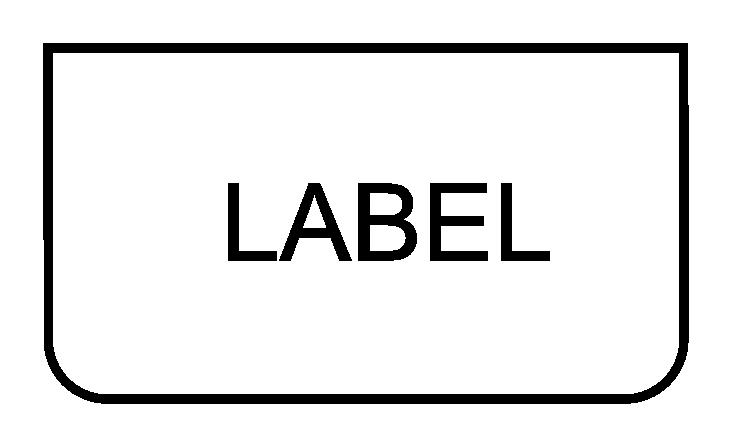
\includegraphics[width = 1.25in]{images/genetic-plain}
  \caption{The \AF glyph for \glyph{nucleic acid feature activity}.}
  \label{fig:af:genetic}
\end{figure} 